\documentclass[a4paper,10pt]{article}
\usepackage[utf8]{inputenc}
\usepackage[T1]{fontenc}
% Use correct language package
\usepackage[british]{babel}
\selectlanguage{british}
% Sets page size and margins
\usepackage[top=1.8cm, bottom=1.8cm, left=2cm, right=2cm]{geometry}
% Use multi-line comments
\usepackage{comment}
% math symbols etc.
\usepackage{amsmath}
% making pictures
\usepackage{graphicx}
% making enumerations
\usepackage{enumitem}
% making an appendix
\usepackage{appendix}
% make a wrap figure
\usepackage{wrapfig}
% align caption
\usepackage{caption}

\begin{document}

\section*{Context and theory of this experiment}

\subsection*{Thermal Expansion Reading Michelson Interferometer Testing Experiment \\ (TERMITE)}
The Michelson Interferometer uses in it simplest form only 5 optical elements (see figure \ref{fig:1} a) ). Light from a laser, in our case a red laser diode, is directed at the beam splitter. Here half of the laser light is transmitted to mirror 2 and the other half is reflected to mirror 1. The two separated beams will be reflected at the mirrors and the light will recombine at the beam splitter. Here once again half is reflected and half is transmitted, but this time both light beams go towards the light detector. If both mirrors have the same distance to the beam splitter the recombination gives a fringe pattern on the detector with a circular light spot surrounded by a dark ring. This ring is followed by a light ring and another dark ring and so forth.

This also works if the difference of the pathlength from a mirror to the beam splitter is exactly one wavelength difference. If it is half a wavelength difference the pattern will be inverted, and if the pathlength changes over time you will cycle through these two patterns. One of these cycles corresponds exactly to one wavelength of your light source. This phenomenon is exactly what we will try to use in our experiment to measure changes in pathlength.\\

\noindent The idea is simple:\\
1.	Fix all the optical elements except one mirror.\\
2.	Allow this mirror to move and thereby change its pathlength to the beam splitter.\\
3.	Measure how many times you went through a cycle of the fringe pattern for a given measurement period.\\
4.	Use this information to compute how much the pathlength has changed over that measurement period.\\

\noindent We wanted to build and design a setup for this concept and decided to measure the thermal expansion of a metal sample for our proof of concept. The design would have all elements fixed with one mirror attached to a metal sample that could be heated/cooled to make it expand or shrink. This will introduce the pathlength difference into our Interferometer, as shown in figure \ref{fig:1} b). By adding a simple temperature sensor we can then compare the expansion to the temperature difference and make a simple measurement of the thermal expansion coefficient for the sample.


\begin{figure}[h]
    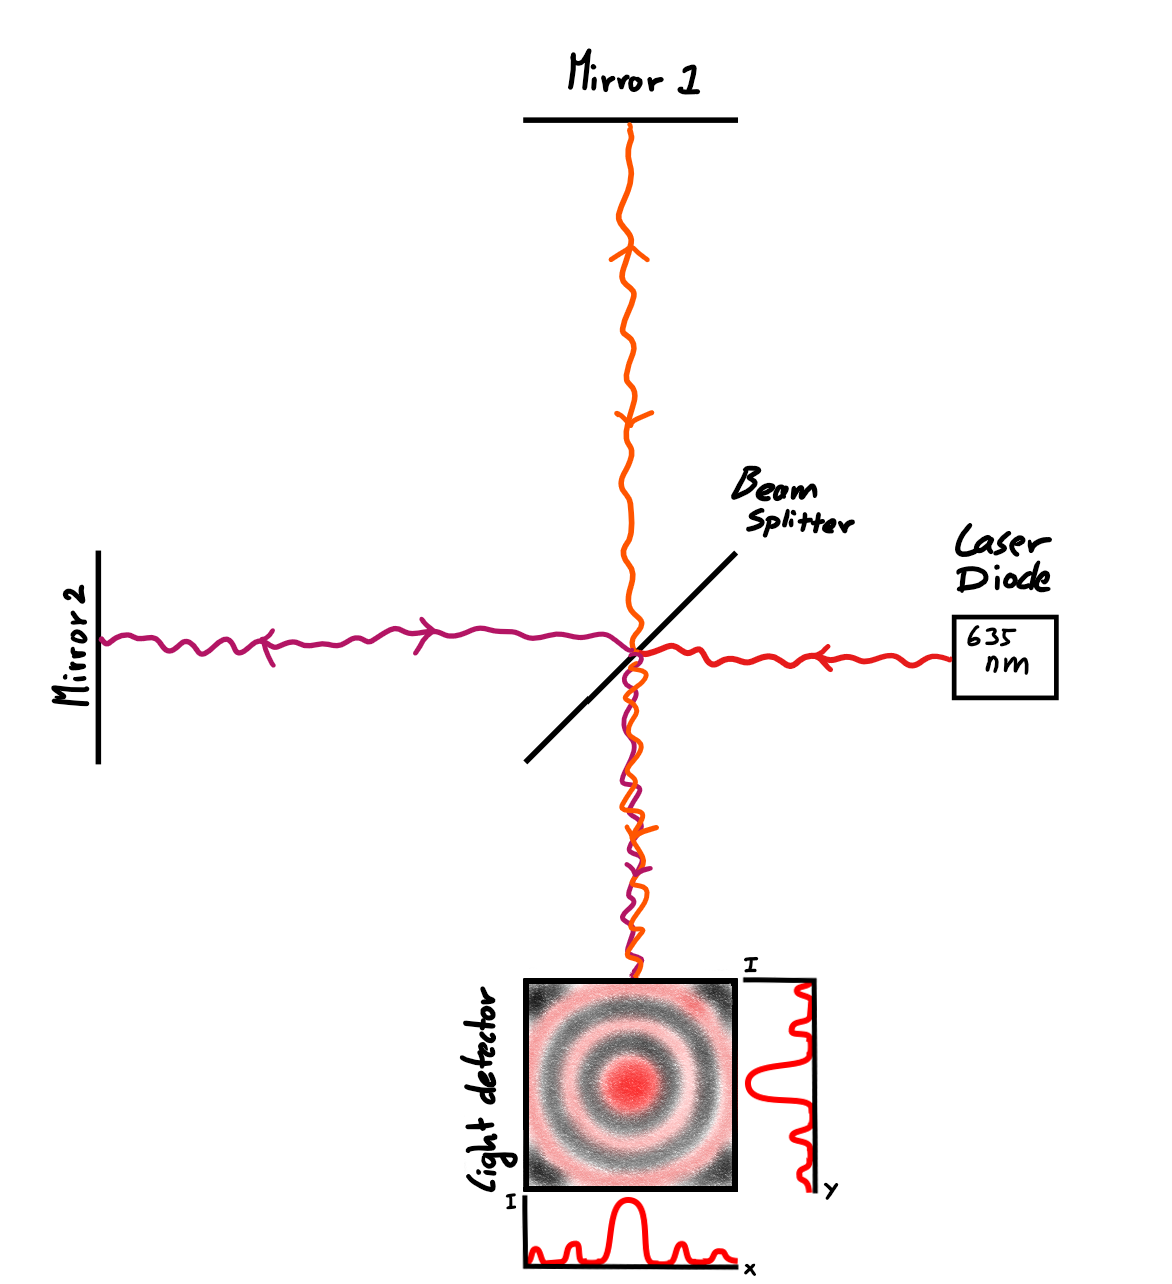
\includegraphics[width=0.49\textwidth]{M_Interferometer2.PNG}
    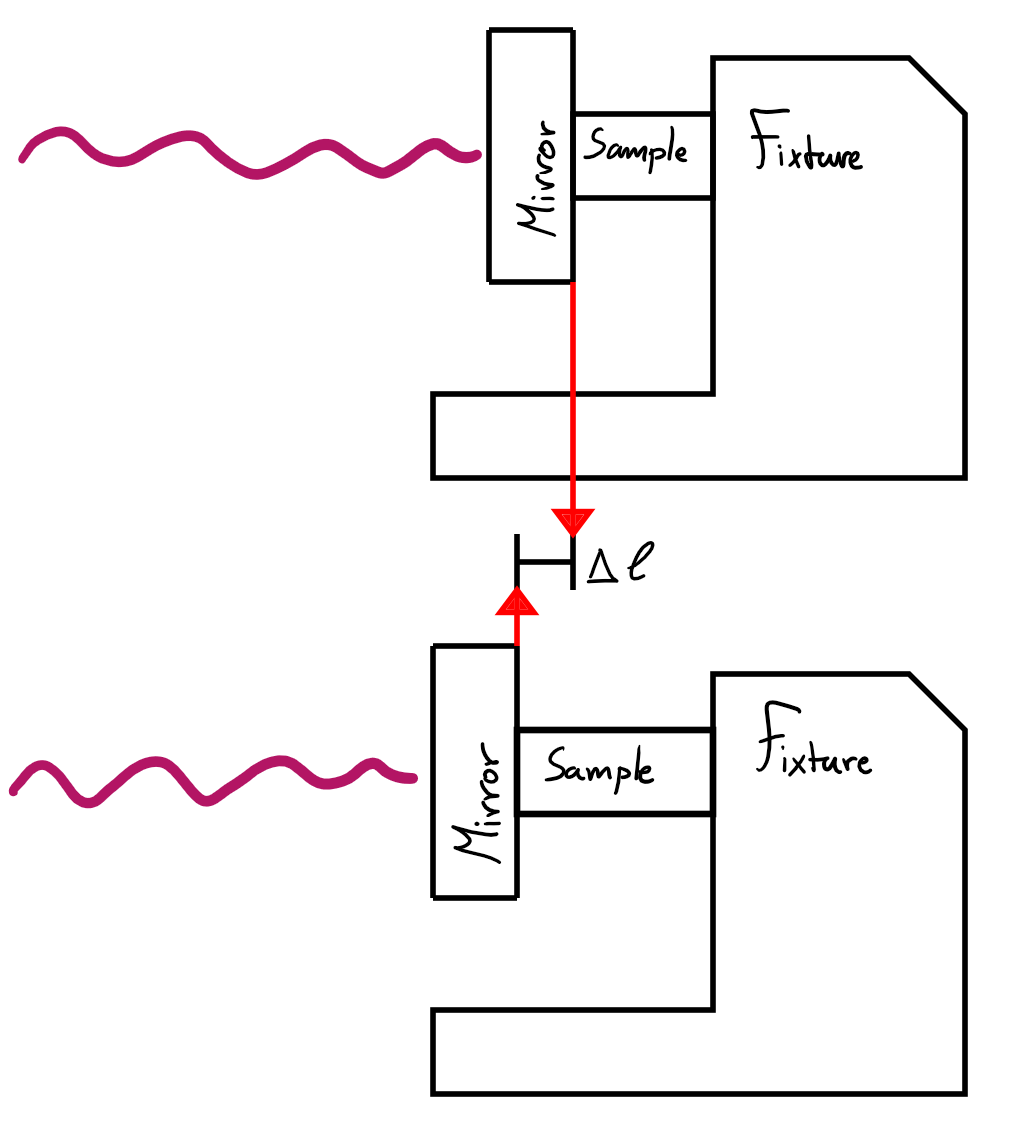
\includegraphics[width=0.49\textwidth]{Sample_Mirror.PNG}
    \caption{a) An example of the simplest form of an Michelson Interferometer. b) Example of how the thermal expansion of a sample can change the pathlength for one of the Michelson Interferometer mirrors. Note that $\Delta\:l$ is the expansion distance and therefor also pathlength difference.}
    \label{fig:1}
\end{figure}

\end{document}
